\section{Fundamentos de Mapas Web}
	
	\subsection{Coordenadas Geográficas}
	Coordenadas geográficas são usadas para expressar localizações no mundo. Existem vários sistemas de coordenadas diferentes. O usado pelo Google Maps é o Word Geodetic System 84 (WGS84), que é o mesmo sistema que o Global Position System(GPS) usa.
	
	As coordenadas são expressas usando o conceito de latitude e longitude. Onde latitude mede do sul ao norte e longitude mede do oeste para o leste. No equador a latitude é 0. Isso significa que tudo abaixo do equador (hemisfério sul) possui uma latitude negativa, e tudo acima possui uma latitude positiva. Similarmente também existe uma linha zero para longitude. É conhecida como meridiano, e por razões históricas passa por Greenwich, Inglaterra. Cada posição que é localizada a leste desta linha tem um número positivo e tudo a oeste tem um número negativo\cite[4]{livroGoogleApiV3}. 
	
	A \autoref{fig-coordenadas} permite uma melhor observação desses conceitos:
	\begin{figure}[htb]
	\caption{\label{fig-coordenadas} O centro do mundo na latitude 0 e longitude 0 reside em algum lugar a oeste da costa da África}
	\begin{center}
	    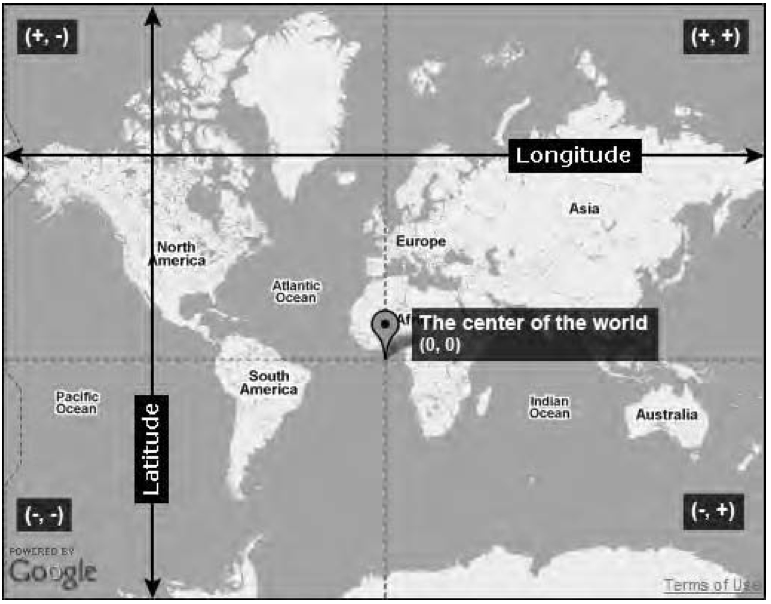
\includegraphics[scale=0.5]{goo-coordenadas}
	\end{center}
	\legend{Fonte: \cite[5]{livroGoogleApiV3}}
	\end{figure}
	
	Dessa forma é possível representar o mapa do mundo em uma imagem retangular que é projetada sobre o plano cartesiano.
	
	Caso seja necessário um maior grau de detalhamento, do mapa, basta que se aumente a resolução da imagem mantendo as proporções e relações entre as coordenadas (x,y), do plano cartesiano, com as coordenadas (longitude, latitude) que são usadas pelo mapa.
		
	\subsection{Zoom}
	As coordenadas de longitude e latitude servem para localizar um ponto numa imagem retangular, através de suas correspondentes x e y do plano cartesiano. Porém mapas também fornecem uma terceira coordenada conhecida como coordenada de Zoom.
	
	 Esta  coordenada controla qual o tamanho da imagem que será usada para projetar o mapa sobre o plano cartesiano. Usualmente, um mapa com coordenada zoom, ou nível de zoom, igual a zero possui uma imagem de tamanho 256x256 pixels. A cada incremento, da coordenada de zoom, dobra-se o tamanho da imagem usada para representar o mapa, e consequentemente o nível de detalhes. De forma que  para zoom=1 a imagem terá 512x512 pixels, para zoom=2 terá 1024x1024 e assim por diante. A \autoref{fig-zoomlevels} exemplifica esse processo:
	\begin{figure}[htb]
	\caption{\label{fig-zoomlevels} A cada incremento de zoom um mapa dobra a sua resolução de imagems}
	\begin{center}
	    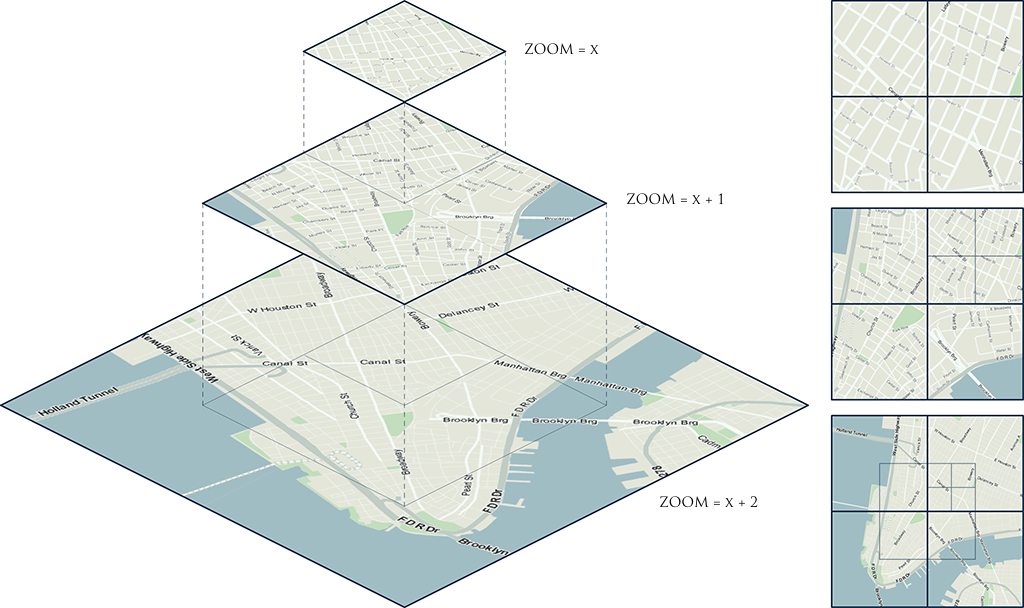
\includegraphics[scale=0.45]{tiles3d}
	\end{center}
	\legend{Fonte: http://workshops.opengeo.org/suiteintro/geowebcache/basics.html}
	\end{figure}

	Portanto para localizar uma posição  em um mapa web, de forma detalhada, precisamos de 3 coordenadas: latitude, longitude e zoom. Além disso, como o tamanho da imagem da projeção varia de acordo com o nível de zoom, o mapa precisa ajustar os valores das coordenadas latitude e longitude para que mantenham suas proporções para os diversos níveis de zoom.

\section{Estratégias para lidar com muitos marcadores}
	Um problema comum, ao se trabalhar com mapas de crowdsourcing, é a enorme quantidade de marcadores necessários para representar os dados do mapa. Isto geralmente afeta a performance do mapa, pois quanto mais marcadores são inseridos mais lenta fica a exibição do mapa. 
	
	É difícil calcular exatamente qual o número máximo de marcadores que um mapa suporta antes de começar a ficar lento, pois a velocidade de exibição do mapa depende tanto do navegador quando do computador em que é exibido. Por exemplo, um mapa pode ser exibido bem rápido em um navegador como o Google Chrome e ao mesmo tempo ser lento quando exibido no Internet Explorer.\cite[177]{livroGoogleApiV3}
	
    Portanto, é necessário um estudo sobre as  estratégias para se lidar com o problema de exibição de muitos marcadores em um mapa. Em \cite[capítulo~9]{livroGoogleApiV3} o autor comenta sobre duas estratégias básicas para esse problema. A primeira e mais óbvia é reduzir o número de marcadores. A segunda estratégia consiste em agrupar os marcadores por algum grau de semelhança.
    
  \subsection{Reduzindo o número de marcadores}
  Existem muitos meios de se reduzir o número de marcadores, entre eles destaca-se as reduções via busca, filtro e otimização visual.
	\subsubsection{Busca}
	Para se reduzir  o número de marcadores exibidos no mapa pode-se fornecer um mecanismo de pesquisa ou busca no mapa. Dessa forma mesmo que o mapa possua milhões de marcadores, somente aqueles que satisfaçam os critérios da busca são exibidos.
	
	 \begin{figure}[htb]
	\caption{\label{fig-estrategiabusca}Busca como estratégia para redução do número de marcadores}
	\begin{center}
	    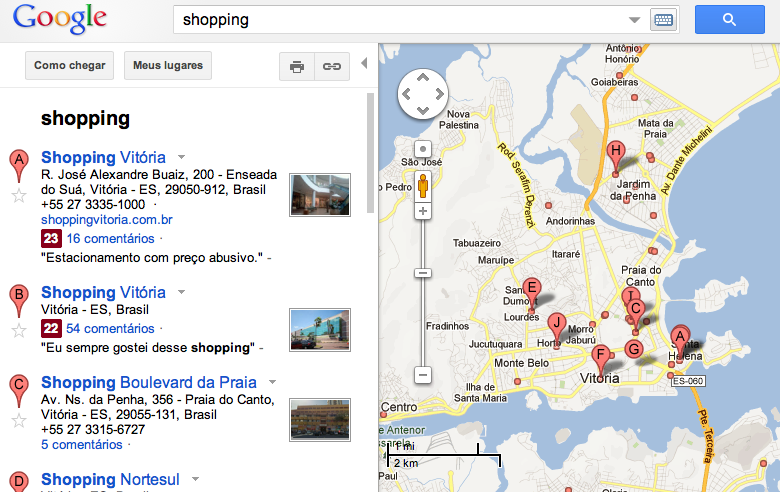
\includegraphics[scale=0.6]{estrategia-busca}
	\end{center}
	\legend{Fonte: http://maps.google.com}
	\end{figure}
	 
	 A \autoref{fig-estrategiabusca}  exemplifica isso ao mostrar o exemplo de busca no google maps. O google maps possui um catálogo enorme de informações, sobre diversas regiões geográficas, mostrar todas essas informações ao mesmo tempo deixaria o mapa muito poluído, e praticamente inutilizável. Como ele implementa o mecanismo de busca isto não acontece.
	
	 Na \autoref{fig-estrategiabusca} observa-se a exibição de uma busca pela palavra chave shopping. Nesta mesma região de interesse existem estabelecimentos de outras categorias como supermercados, lojas, padarias etc. Mas o google maps exibe apenas os marcadores relativos a categoria shopping, que é a palavra chave da busca. Ao fazer isso o mapa fica mais limpo e compreensivo.
	 
	
	\subsubsection{Filtro}
	De forma similar ao mecanismo de busca, um mapa também pode possuir um mecanismo para filtrar grupos de marcadores de acordo com algum critério de seleção do grupo. Dessa forma somente os marcadores que pertençam aos grupos marcados no filtro são exibidos no mapa. 
	
	Diferente do método de busca, este método permite ser mais específico e direto, pois cada campo do filtro é relacionado diretamente com alguma categoria contida nas informações. No método de busca esta relação é menos direta e depende do algorítimo de busca utilizado.  
	
	Como exemplo, ao utilizar-se do método de filtro para marcar 2 categorias, obrigatoriamente, deve ser retornado o resultado para as duas categorias que foram marcadas. Já com o método de busca isto nem sempre é verdade, pois dependendo do algorítimo de busca ele pode entender que a busca por ``categoria 1 categoria 2'' é uma busca por 2 categorias ou uma busca por uma categoria conhecida como ``categoria 1 categoria 1'', que obviamente não seria encontrada. 
	
	A \autoref{fig-estrategiafiltro} mostra um mapa com filtro a esquerda. Observa-se que apenas os marcadores dos grupos  ``Student Housing'' e ``Food/Dining''  são exibidos no mapa.
	 \begin{figure}[htb]
	\caption{\label{fig-estrategiafiltro}Filtro como estratégia para redução do número de marcadores}
	\begin{center}
	    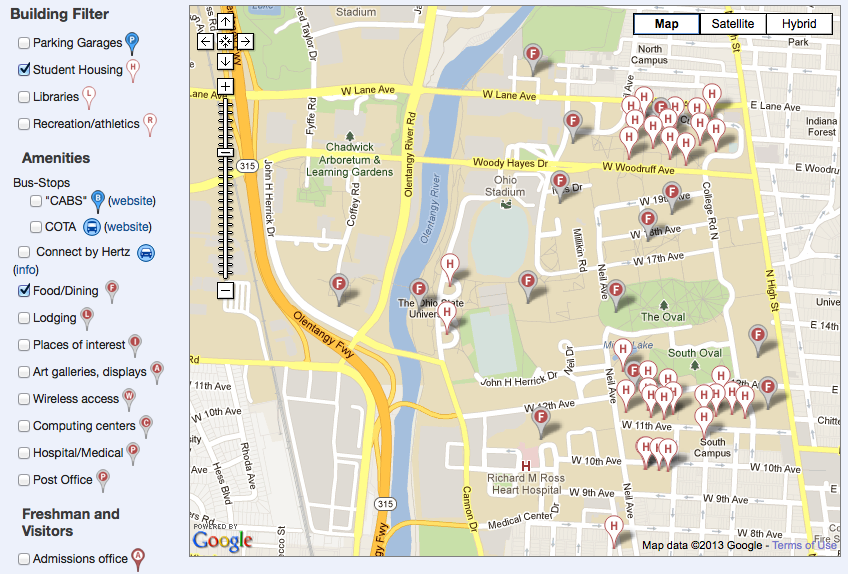
\includegraphics[scale=0.5]{estrategia-filtro}
	\end{center}
	\legend{Fonte: http://www.osu.edu/map/google.php}
	\end{figure}
	 
	\subsubsection{Otimização Visual}
	Nem sempre é preciso usar marcadores para representar dados de um mapa. Em alguns mapas faz mais sentido usar polígonos ou grupo de polígonos para representar um dado ao invés de simplesmente um ponto para o marcador. Por exemplo, ao exibir uma rota  não é necessário um marcador para cada vértice da rota, pois precisa-se apenas do desenho de uma linha, passando por cada vértice, para que a rota seja representada.
	
	A \autoref{fig-otimizacao} mostra um exemplo desse tipo de otimização. No mapa à esquerda, ela exibe uma rota com marcadores em cada vértice do trajeto percorrido. No mapa à direita, ela exibe a mesma rota só que sem colocar marcadores nos vértices do trajeto, deixando apenas um marcador para exibir o ponto de início do trajeto.
	
	 \begin{figure}[htb]
	\caption{\label{fig-otimizacao}Otimização Visual como estratégia para redução do número de marcadores}
	\begin{center}
	    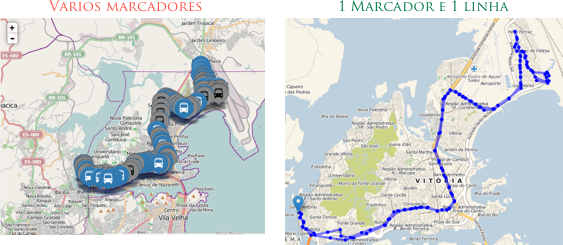
\includegraphics[scale=0.7]{estrategia-otimizacao}
	\end{center}
	\end{figure}
	
	Nesse exemplo, cada vértice da rota representa um ponto de parada para os ônibus que percorrem esse trajeto. Inicialmente, pode se achar necessário a exibição de marcadores nesses vértices como mecanismos de interação com os dados que eles representam. Por exemplo, os usuários do transporte público poderiam querer saber quais são os horários que determinados ônibus passam naquele ponto específico, e com um simples clique no marcador o mapa poderia exibir essa informação. 
	
	Porém, para que este tipo de interação seja possível o mapa teria que exibir os marcadores em cada vértice, que como mostrado na \autoref{fig-otimizacao} não é o melhor caminho. Felizmente existem alternativas para esse processo que não exigem a presença de um marcador, por exemplo ao clicar na linha da rota o mapa pode fazer uma busca, baseada em proximidade, e localizar o ponto que o usuário deseja saber mais informações. Após isso o mapa pode até exibir um marcador temporário como reforço visual do local que está sendo exibida a informação.
	

  \subsection{Agrupamento/Clustering}
  pagina 199 (google)
  
  	 
 pagina 198

 
 (pagina 88 ,silva, tabela 6, figura 93, figura 65 ())
ss
		\subsubsection{Por grelha}
		\subsubsection{Por distancia}
		\subsubsection{Por região}
		
\section{Algorítimos de agrupamento}
	\subsection{Métodos baseados em grelha}
		\subsubsection{WaveCluster}
	\subsection{Aplicações}
		\subsubsection{MarkerCluster}
		pagina 206 a 212
		\subsubsection{MarkerClustered}



\section{Planilhas eletrônicas e Mapas}
\subsection{O desafio chinês}
mostra o uso de planilhas pelo governo chines \cite{chinaPlanilha}
\subsection{Domínios de conhecimento}
Mostra a importância do uso de planilhas \cite{credinePlanilha} 
\subsection{Usando planilhas como fonte de dados para Mapas Geográficos}
Mostra \cite{lieberman2009spatio}